\section{Storage and snapshots}
\label{sec:storage}

This section details the storage layer and the snapshot mechanism as implemented in
\code{src/storage/} and \code{src/raft/snapshot.rs}, identifies the risks of running it in
production, and proposes a redesign ordered by priority.

\subsection{The \code{Storage} contract}

The engine accesses persistence only through the \code{Storage} trait (generic
\code{RaftEngine<S: Storage>}), so backends can be swapped without touching Raft logic.

\begin{center}
\begin{tabular}{@{}L{0.36\linewidth}L{\restwidth{0.36\linewidth}}@{}}
\toprule
\textbf{Method} & \textbf{Meaning and constraints} \\
\midrule
\code{hard\_state()} & Current \code{current\_term} and \code{voted\_for}. \\
\code{first\_index()} & First index still in the log: \code{last\_included\_index + 1}, or 1 if there is no snapshot. \\
\code{entry(i)} & Entry at index \code{i}; \code{None} if compacted away or not yet present. \\
\code{last\_index\_term()} & \code{(index, term)} of the last entry; taken from the snapshot if the log is empty. \\
\code{truncate\_from(i)} & Delete entries from \code{i} onwards (follower conflict). \\
\code{persist(hs, entries)} & Write the hard state (if any) and append/overwrite entries in \emph{one} call; returns \code{Result}. \\
\code{snapshot()} & The current snapshot (returned as a copy). \\
\code{install\_snapshot(snap)} & Store the snapshot and compact the log prefix; ignores snapshots older than the current one. Returns no error. \\
\bottomrule
\end{tabular}
\end{center}

\subsection{Data model}

\begin{lstlisting}
pub struct HardState { pub current_term: Term, pub voted_for: Option<NodeId> }

pub struct Snapshot {
    pub last_included_index: Index,  // last entry reflected in state_blob
    pub last_included_term: Term,
    pub conf: Vec<NodeId>,           // voter set at snapshot time
    pub state_blob: Vec<u8>,         // state machine serialized by the app
}
\end{lstlisting}

After compaction the log is only a contiguous \emph{suffix} starting at \code{first\_index}.
Every entry with index $\le k$ (\code{last\_included\_index}) is considered committed and applied.

\begin{figure}[H]
\centering
\begin{tikzpicture}[
  cell/.style={draw=black!45, minimum width=1.3cm, minimum height=0.75cm, font=\small},
  ptr/.style={-{Stealth[length=1.8mm]}, semithick, draw=black!70},
  ptrlbl/.style={font=\scriptsize, align=center}]
\node[draw=brand!60, fill=brand!10, minimum width=4.2cm, minimum height=0.75cm,
      font=\small, align=center] (snap) at (2.1,0) {Snapshot\\[-1pt]{\scriptsize indices $1..k$ (compacted)}};
\foreach \i/\t/\f in {0/{$k{+}1$}/black!5, 1/{$k{+}2$}/black!5, 2/{$\ldots$}/black!5, 3/{$c$}/black!5,
                      4/{$\ldots$}/white, 5/{$n$}/white} {
  \node[cell, fill=\f] (c\i) at (4.2+0.65+1.3*\i,0) {\t};
}
\draw[ptr] (c0.north) ++(0,0.55) node[ptrlbl, above] {\code{first\_index}} -- (c0.north);
\draw[ptr] (c3.north) ++(0,0.55) node[ptrlbl, above] {\code{commit\_index}} -- (c3.north);
\draw[ptr] (c5.north) ++(0,0.55) node[ptrlbl, above] {\code{last\_index}} -- (c5.north);
\draw[decorate, decoration={brace, mirror, amplitude=4pt}, draw=black!60]
  ([yshift=-3pt]c0.south west) -- ([yshift=-3pt]c3.south east)
  node[midway, below=5pt, ptrlbl] {committed, awaiting the next snapshot};
\draw[decorate, decoration={brace, mirror, amplitude=4pt}, draw=black!60]
  ([yshift=-3pt]c4.south west) -- ([yshift=-3pt]c5.south east)
  node[midway, below=5pt, ptrlbl] {uncommitted};
\end{tikzpicture}
\caption{Log layout after compaction: the snapshot replaces prefix $1..k$; the log keeps suffix $k{+}1..n$.}
\end{figure}

\code{install\_snapshot} follows Section 7 of the Raft paper~\cite{ongaro2014raft}: if the log
holds an entry at $k$ whose term matches \code{last\_included\_term}, the suffix after $k$ is
retained; otherwise the whole log is discarded.

\subsection{The two existing backends}

\begin{center}
\begin{tabular}{@{}L{0.22\linewidth}L{0.36\linewidth}L{\dimexpr0.42\linewidth-4\tabcolsep\relax}@{}}
\toprule
\textbf{Data} & \textbf{\code{MemoryStorage}} & \textbf{\code{FileSnapshotStorage}} \\
\midrule
Hard state & RAM & RAM \\
Log entries & RAM (\code{Vec} from \code{first\_index}) & RAM (wraps \code{MemoryStorage}) \\
Snapshot & RAM & RAM + file \code{snapshot.bin} (bincode) \\
File write & --- & Temp file, \code{fsync}, \code{rename} (atomic replace) \\
After crash/restart & Everything lost & Only the snapshot survives; hard state and log tail are lost \\
Used by & Unit/integration tests & \code{bin/raft-node.rs} (\code{DATA\_DIR}) \\
\bottomrule
\end{tabular}
\end{center}

\subsection{Local compaction}

\begin{enumerate}[label=\arabic*., nosep]
  \item After every apply the engine calls \code{should\_snapshot}: if
    \code{last\_applied - last\_included\_index >= snapshot\_threshold} it emits
    \code{Action::SnapshotNeeded \{ last\_applied \}} (the \code{snapshot\_requested} flag prevents repeats).
  \item The behaviour turns it into \code{Event::SnapshotNeeded} for the application.
  \item The application serializes its state machine as of \code{last\_applied} and calls
    \code{behaviour.compact(index, blob)}.
  \item \code{RaftEngine::compact} checks \code{0 < index <= last\_applied}, looks up the term at
    \code{index}, builds \code{conf} from the current membership, and calls \code{storage.install\_snapshot}.
\end{enumerate}

\code{raft-node} sets \code{snapshot\_threshold} to 10\,000 but has no state machine: on
\code{SnapshotNeeded} it only logs and never calls \code{compact}.

\subsection{Leader $\rightarrow$ follower snapshot transfer}

When \code{next\_index[F] < first\_index}, the leader no longer has the entries needed for
AppendEntries and switches to \code{InstallSnapshot}. The \code{state\_blob} is cut into chunks of
\code{DEFAULT\_SNAPSHOT\_CHUNK\_SIZE = 64 KiB}, with only \textbf{one} chunk in flight per follower.

\begin{figure}[H]
\centering
\begin{tikzpicture}
\seqactors{-8.5}{0/Leader engine, 6.3/Follower engine, 12.6/Follower app}
\seqnote{0}{-0.95}{\code{next\_index[F]}\\ \code{< first\_index}}
\seqmsg{0}{6.3}{-1.85}{\code{InstallSnapshot} (offset 0, 64 KiB, \code{done=false})}
\seqnote{6.3}{-2.5}{\code{InboundAssembly::accept} $\rightarrow$ Partial}
\seqmsg[seqret]{6.3}{0}{-3.15}{\code{InstallSnapshotResp \{ term \}}}
\seqnote{0}{-3.8}{\code{offset += len}}
\seqmsg{0}{6.3}{-4.55}{\ldots{} last chunk (\code{done=true})}
\seqnote{6.3}{-5.35}{Complete $\rightarrow$ \code{install\_snapshot}\\ \code{commit\_index = last\_applied = k}}
\seqmsg{6.3}{12.6}{-6.2}{\code{Event::SnapshotInstalled}}
\seqmsg[seqret]{6.3}{0}{-6.85}{\code{InstallSnapshotResp \{ term \}}}
\seqnote{0}{-7.75}{\code{match\_index = k}\\ \code{next\_index = k+1}\\ $\rightarrow$ AE for the tail}
\end{tikzpicture}
\caption{Chunked snapshot transfer, one chunk at a time (pipeline depth 1).}
\end{figure}

\textbf{Current error-handling rules:}
\begin{itemize}[nosep]
  \item RPC error or timeout $\rightarrow$ \code{handle\_rpc\_failure} deletes \code{snap\_out[F]}; the next attempt restarts from offset 0 (no resume).
  \item The leader's local snapshot changes mid-transfer $\rightarrow$ restart from offset 0.
  \item The follower receives a chunk with \code{offset = 0} $\rightarrow$ drops its buffer and starts a new transfer; a chunk with a wrong offset or wrong \code{(index, term)} $\rightarrow$ \code{Rejected}, buffer reset.
  \item A snapshot with \code{last\_included\_index <= commit\_index} on the follower $\rightarrow$ content ignored, a response is still sent.
\end{itemize}

\textbf{Throughput:} one chunk per round trip, i.e.\ $\approx$ \code{64 KiB / RTT}. At 1\,ms RTT
that is about 64\,MiB/s; at 50\,ms RTT only about 1.3\,MiB/s, so a 1\,GiB snapshot takes about
14 minutes.

\subsection{Recovery on startup}

\begin{enumerate}[label=\arabic*., nosep]
  \item \code{FileSnapshotStorage::new(dir)} creates the directory and reads \code{snapshot.bin} if
    present; a corrupt file (decode error) returns \code{StorageError} instead of silently resetting.
  \item \code{RaftEngine::new} sets \code{commit\_index = last\_applied = first\_index - 1}
    (everything in the snapshot counts as applied).
  \item The hard state is reset to default (term 0, no vote) and the log is empty; the node rejoins as a
    follower and the leader fills in the tail via AppendEntries or a snapshot.
  \item The application must rebuild its state machine from \code{snapshot.state\_blob};
    \code{raft-node} currently only prints the snapshot size.
\end{enumerate}

\subsection{Production risks}

\begin{center}
\begin{tabular}{@{}L{0.05\linewidth}L{0.33\linewidth}L{\dimexpr0.62\linewidth-4\tabcolsep\relax}@{}}
\toprule
\textbf{\#} & \textbf{Issue} & \textbf{Consequence} \\
\midrule
R1 & Hard state not durable & A node votes for A in term 5, crashes, restarts with term 0 and then votes for B in term 5 too $\rightarrow$ two leaders in one term become possible (violates election safety). \\
R2 & Log tail not durable & A follower acknowledges \code{AppendEntriesResp} success while the entry is only in RAM. If a majority loses power at once, a committed entry (possibly already reported to a client) is lost. \\
R3 & Storage errors are swallowed & The engine calls \code{let \_ = storage.persist(..)}; \code{install\_snapshot} returns no \code{Result} and only logs. The node keeps running with state that diverges from disk. \\
R4 & No \code{fsync} of the directory after \code{rename} & On ext4/XFS a power loss right after \code{rename} can lose the new snapshot. \\
R5 & Snapshot file has no header & No magic, version or checksum; a bincode format change or bit rot cannot be detected or migrated. \\
R6 & Whole snapshot cloned per chunk & \code{send\_snapshot\_chunk\_to} calls \code{storage.snapshot()} (which returns a copy) for \emph{every} chunk: a 1\,GiB snapshot with 64\,KiB chunks $\Rightarrow$ 16\,384 copies of 1\,GiB. \\
R7 & Whole blob held in RAM & The leader keeps the blob inside \code{Snapshot}, the follower assembles it in a \code{Vec}; state larger than RAM is infeasible. \\
R8 & Response cannot signal rejection & \code{InstallSnapshotResp} only carries \code{term}: a \code{Rejected} chunk is still counted as received by the leader. The system self-heals via a rejected AppendEntries, but wastes a full transfer. \\
R9 & \code{conf} is not sent on the wire & The follower records \code{conf} from its own membership, not from the leader's snapshot. \\
R10 & Synchronous serialization & Applications typically call \code{compact} inside the Swarm loop; a large state blocks the event loop, delays heartbeats and can trigger spurious elections. \\
R11 & Low throughput & One 64\,KiB chunk per RTT, no window, no resume. \\
\bottomrule
\end{tabular}
\end{center}

\subsection{Production recommendations}

\subsubsection{P0 --- Durability and safety (mandatory)}

\begin{itemize}[nosep]
  \item \textbf{A truly durable backend} (fixes R1, R2): a segmented append-only WAL, or an embedded KV
    store (\code{redb}, \code{sled}, RocksDB). \code{persist(hs, entries)} writes \emph{one atomic batch}
    and \code{fsync}s before returning.
  \item \textbf{Persist before replying:} persist \code{voted\_for} before sending a granted
    \code{RequestVoteResp}; persist entries before sending a successful \code{AppendEntriesResp}.
    The engine already calls storage in this order; only the backend needs to be durable.
  \item \textbf{Fail-stop on storage errors} (R3): every write method returns \code{Result}; on error the
    engine stops participating in the cluster (surfacing the error so the application shuts down) instead of
    continuing with non-durable state.
  \item \textbf{Correct file writes} (R4, R5): \code{fsync} the parent directory after \code{rename}; give
    the snapshot file a \code{magic | version | len | crc32c} header and keep the previous file until the
    new one is durable.
\end{itemize}

\begin{lstlisting}
// Proposed: explicit errors + streaming snapshot I/O
pub trait Storage {
    fn persist(&mut self, hs: Option<HardState>, entries: &[LogEntry])
        -> Result<(), StorageError>;                 // atomic + fsync
    fn truncate_from(&mut self, index: Index) -> Result<(), StorageError>;
    fn snapshot_meta(&self) -> Option<SnapshotMeta>; // index, term, conf, len, crc
    fn read_snapshot_chunk(&self, offset: u64, len: usize)
        -> Result<Vec<u8>, StorageError>;
    fn begin_snapshot_install(&mut self, meta: SnapshotMeta)
        -> Result<Box<dyn SnapshotSink>, StorageError>; // writes to a temp file
}
\end{lstlisting}

\subsubsection{P1 --- Non-blocking snapshots and streaming transfer}

\begin{itemize}[nosep]
  \item \textbf{Asynchronous snapshot creation} (R10): the application captures a consistent view at
    \code{last\_applied} (immutable data structures, copy-on-write, or a DB checkpoint), serializes it in
    \code{spawn\_blocking}, and only then calls \code{compact(index, ..)}. The engine keeps running meanwhile.
  \item \textbf{Read chunks from a file} (R6, R7): the leader reads by \code{offset} from the snapshot file
    instead of cloning the blob; the follower writes each chunk to a temp file, verifies the checksum,
    \code{fsync}s, \code{rename}s, and only then installs.
  \item \textbf{Extend the wire format} (R8, R9):
    \code{InstallSnapshotResp \{ term, success, next\_offset \}} for explicit rejection and resume;
    the first chunk carries \code{conf}, \code{total\_len} and \code{crc32c}.
  \item \textbf{Keep some log after the snapshot} (\code{trailing\_logs}): a follower that is only slightly
    behind still gets AppendEntries rather than a full snapshot.
\end{itemize}

\subsubsection{P2 --- Performance and operations}

\begin{itemize}[nosep]
  \item \textbf{Throughput} (R11): a window of $N$ chunks in flight, or a dedicated libp2p substream that
    streams the whole snapshot with backpressure; chunks of 256\,KiB--1\,MiB (below
    \code{MAX\_FRAME\_BYTES} = 4\,MiB); rate limiting so snapshot traffic does not crowd out heartbeats.
  \item \textbf{A byte-based threshold} in addition to the entry count, so logs with large entries are
    compacted in time.
  \item \textbf{Metrics:} snapshot size and creation time, bytes transferred, retransmissions,
    \code{fsync} latency.
  \item \textbf{Testing:} one \code{Storage} contract test suite shared by every backend; crash tests
    (\code{kill -9} during \code{persist} and during a snapshot write); Jepsen-style fault injection for
    simultaneous power loss on a majority of nodes.
\end{itemize}

\begin{invariantbox}[Priority order]
P0 is the precondition for calling the system crash-safe Raft; without P0 every guarantee holds only if
no node ever restarts. P1 is needed once the state machine grows beyond a few tens of MiB. P2 is
optimisation for real deployments.
\end{invariantbox}
